%%%%%%%%%%%%%%%%%%%%%%%%%%%%%%%%%%%%%%%%%%%%%%%%%%%%%%%%%%%%%%%%%%%%%%%%%%
%%%%%%%%%%%%   CAPTER   %%%%%%%%%%%%%%%%%%%%%%%%%%%%%%%%%%%%%%%%%%%%%%%%%%
%%%%%%%%%%%%%%%%%%%%%%%%%%%%%%%%%%%%%%%%%%%%%%%%%%%%%%%%%%%%%%%%%%%%%%%%%%
\chapter{Block Diagrams}
\label{chap:appendix}

\section{Nitrogen6X Development Kit}
\label{app:nitrogen6x}

\begin{figure}[h!]
	\centering
	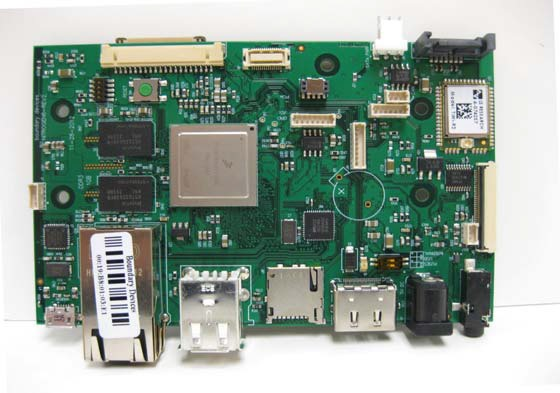
\includegraphics[]{figures/nitrogen6x}
	\caption{Nitrogen6X Development Kit \cite{nitrogen6x}}
	\label{fig:app:nitrogen6x}
\end{figure}
\newpage

\section{iMX6Quad CPU}
\label{app:imx6q}

\begin{figure}[h!]
	\centering
	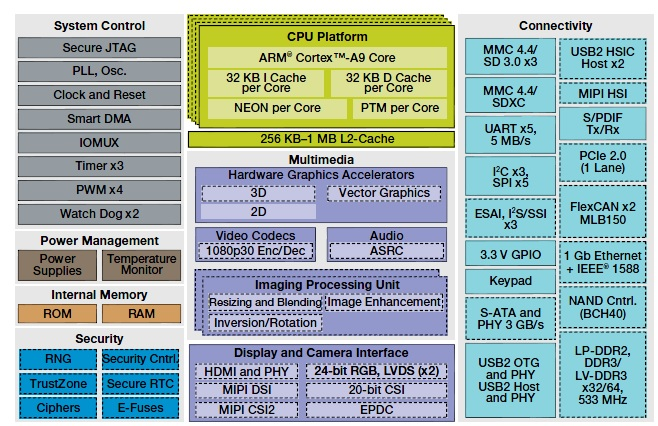
\includegraphics[width=160mm, height=110mm]{figures/imx6q}
	\caption{Internals of iMX6Quad CPU \cite{imx_spec}}
	\label{fig:app:imx6q}
\end{figure}


\cleardoublepage
\chapter{Description of the Benchmark Functions}
\label{description:benchmark}
\begin{longtable}{rp{120mm}}
	\hypertarget{benchmarks}{100CMYACC8:}& Multiply each element of a 100 x 8-element complex matrix with an 8-element complex vector and accumulate the 8 complex multiplication results to a single complex result, resulting in a 100 x 1-element complex matrix. \\[0.2cm]
	100RMY50: & Multiply each vector in a 100 x 50-element complex matrix with a 50-element float vector, resulting in a 100 x 50-element complex matrix.\\[0.2cm]
	100CONV64: & Perform fast convolution of a 100 x 64-element complex matrix: complex 64-pt FFT, followed by a multiplication with a 64-element float vector, followed by a 64-pt complex inverse FFT, resulting in a 100 x 64-element complex matrix. \\[0.2cm]
	150COT50: & Perform a corner turning of a 150 x 50 complex matrix into a 50 x 150 complex matrix incl. zero-padding of the elements from 150 to 256\\ [0.2cm]
	50MAG256: & Perform with a 50 x 256-element complex matrix a magnitude square-root calculation, resulting in a 50 x 256 float matrix. \\[0.2cm]
	64AVG100: & Calculate from a 64 x 100-element float matrix the average within a 5x5 area arround the cell. Resulting in a 64 x 100-element float matrix. \\[0.2cm]
	64CMPR100: & Compare a 64 x 100-element float matrix with a float threshold. If  the threshold is execeeded, the corresponding element in a 64 x 100 boolean matrix shall be set to TRUE, otherwise set to FALSE. \\[0.2cm]
	64DET100: & Calculate Main/Guard comparison with a 64 x 100-element float matrix of the sum-channel and a 64 x 100-element float matrix of the guard-channel. Resulting in a 64 x 100-element boolean matrix. \\[0.2cm]
	1CMY1k: & Multiply a 1 x 1k-element complex matrix with a 1 x 1k-element complex matrix, resulting in a 1 x 1k-element complex matrix.\\[0.2cm]
	10MAGSQ1k: & Perform the magnitude square calculation of 10 x 1k complex matrix, resulting in a 10 x 1k float matrix. \\[0.2cm]
	10ACCOFFSET1k: & Perform the accumulation of the data from 4 separate 10 x 1k-element float matrices. The result shall be a 10 x 640 element float matrix. For the access to the vectors an offset of k * 128 elements shall be used (i.e. Novl = 128), where k = {0, 1, 2, 3}.\\[0.2cm]
	100LOG256: & Perform a 10*log10 calculation of the data from 100 x 256-element float matrix, resulting in a 100 x 256-element float matrix. \\[0.2cm]	
	100LIM256: & Perform the upper-limitation of the data of a 100 x 256-element float matrix to a float constant Dmax. All elements in the matrix which are greater than Dmax shall be set to Dmax. Resulting in a 100 x 256-element float matrix. \\[0.2cm]
	100SCAL256: & Perform the scaling algorithm with a 100 x 256-element float matrix. Resulting in a 100 x 256-element byte matrix. Assume Ddisp = 256.\\[0.2cm]
\end{longtable}

\cleardoublepage
%%%%%%%%%%%%%%%%%%%%%%%%%%%%%%%%%%%%%%%%%%%%%%%%%%%%%%%%%%%%%%%%%%%%%%%%%%
%%%%%%%%%%%%   CAPTER   %%%%%%%%%%%%%%%%%%%%%%%%%%%%%%%%%%%%%%%%%%%%%%%%%%
%%%%%%%%%%%%%%%%%%%%%%%%%%%%%%%%%%%%%%%%%%%%%%%%%%%%%%%%%%%%%%%%%%%%%%%%%%
\chapter{Code Snippets}
\label{app:code}

\section{set\_core\_affinity()}
\label{app:code:core_affinity}

\lstset{ %
  backgroundcolor=\color{mildyellow},
  basicstyle=\ttfamily\small,
  breakatwhitespace=false,
  breaklines=true,
  captionpos=b,
  commentstyle=\color{mygreen},
  keepspaces=true,
  keywordstyle=\color{blue},
  otherkeywords={cpu\_set\_t,pthread\_t},
  numbers=left,
  numberstyle=\tiny\color{mygray},
  frame=single,
  showspaces=false,
  showstringspaces=false,
  stringstyle=\color{mymauve},
  language=C
}

\begin{lstlisting}[caption=Set core affinity of calling thread]
int set_core_affinity(int core_id)
{
  int num_cores = sysconf(_SC_NPROCESSORS_ONLN);
  if (core_id < 0 || core_id >= num_cores)
    return CPU_AFFINITY_ERROR;

  cpu_set_t cpuset;
  CPU_ZERO(&cpuset);
  CPU_SET(core_id, &cpuset);

  pthread_t current_thread = pthread_self();
  if(pthread_setaffinity_np(current_thread, sizeof(cpu_set_t), &cpuset) != 0) 
    return CPU_AFFINITY_ERROR;

  return CPU_AFFINITY_OK;
}
\end{lstlisting}


\newpage
\section{wait\_for\_all\_threads()}
\label{app:code:wait_for_others}

\begin{lstlisting}[caption=Wait for other threads to join]
void wait_for_all_threads()
{
  while(awakenedThreads%NUM_THREADS != 0)
    sleep(0.001);

  pthread_mutex_lock(&mutex);
  readyThreads += 1;

  if(readyThreads == NUM_THREADS) {
    pthread_cond_broadcast(&cv_count);
  }

  while(readyThreads != NUM_THREADS)
    pthread_cond_wait(&cv_count, &mutex);

  ++awakenedThreads;
  if(awakenedThreads == NUM_THREADS){
    awakenedThreads = 0;
    readyThreads = 0;
  }

  pthread_mutex_unlock(&mutex);
}
\end{lstlisting}

\lstset{ %
  language=bash
}
\newpage
\section{mem\_util.sh}
\label{app:code:mem_util}
\begin{lstlisting}[caption=Peak Memory Utilization]
#!/bin/bash
ITER=1
PEAK_MEM=0
MEM_SIZE=`free -m | sed -n '2p'| awk '{print $2}'`
DATE_BEGIN=$(date +%Y-%m-%d" "%H:%M:%S)
OUTPUT_FILE="logs/peak_mem_util.csv"

echo "DATE BEGIN,${DATE_BEGIN}" > ${OUTPUT_FILE}

# Check for user input
if [ "$#" = "0" ]
then
# Read from file
PID=`cat logs/pid`
else
PID=$1
fi
echo "PID = ${PID}"

NAME=`cat /proc/${PID}/cmdline`
echo "Application name, ${NAME}" >> ${OUTPUT_FILE}
RES=`eval top -b -n ${ITER} | grep ${PID}`

while [ ! -z "$RES"  ]
do
#echo "res = ${RES}"
array=($RES)
PEAK_MEM=${array[9]}
echo "${PEAK_MEM}" >> ${OUTPUT_FILE}

#echo "Peak mem = ${PEAK_MEM}"
RES=`eval top -b -n ${ITER} | grep ${PID}`
sleep 0.1
done
\end{lstlisting}
